%%%%%%%%%%%%%%%%%%%% author.tex
%%%%%%%%%%%%%%%%%%%%%%%%%%%%%%%%%%%
%
% sample root file for your "contribution" to a proceedings volume
%
% Use this file as a template for your own input.
%
%%%%%%%%%%%%%%%% Springer
%%%%%%%%%%%%%%%%%%%%%%%%%%%%%%%%%%

\documentclass{svproc}
%
% RECOMMENDED
%%%%%%%%%%%%%%%%%%%%%%%%%%%%%%%%%%%%%%%%%%%%%%%%%
%%
%
\usepackage{graphicx}
\usepackage{marvosym}
\usepackage{amssymb}
\usepackage{cite}
\usepackage{subfig}
% to typeset URLs, URIs, and DOIs
\usepackage{url}
\usepackage{hyperref}
\def\UrlFont{\rmfamily}

\def\orcidID#1{\unskip$^{[#1]}$}
\def\letter{$^{\textrm{(\Letter)}}$}

\begin{document}
\mainmatter              % start of a contribution
%
\title{Comparison of several sequential and parallel derivative-free global optimization algorithms}
%
\titlerunning{Comparison of several optimization methods}  % abbreviated title (for running head)
%                                     also used for the TOC unless
%                                     \toctitle is used
%
\author{Vladislav Sovrasov\letter \and Semen Bevzuk}
%
\authorrunning{Vladislav Sovrasov et al.} % abbreviated author list (for running head)
%
%%%% list of authors for the TOC (use if author list has to be modified)
\tocauthor{Vladislav Sovrasov and Semen Bevzuk}
%
\institute{Lobachevsky State University of Nizhni Novgorod, Russia \\
  \email{sovrasov.vlad@gmail.com, semen.bevzuk@gmail.com}
}

\maketitle              % typeset the title of the contribution

\begin{abstract}
This work considers several stochastic and deterministic derivative-free global optimization
algorithms. In the first part of the paper popular sequential open-source solvers are compared against
the Globalizer solver, which is developed at the Lobachevsky State University. The Globalizer is
designed to solve problems with black-box objectives satisfying the Lipschitz condition and shows
competitive performance with other similar solvers. The comparison is done on several sets of
challenging multi-extremal benchmark functions. The second part of this work is devoted to
comparison between the Globalizer and MIDACO solvers on systems with shared and distributed
memory. MIDACO is a state-of-the-art global solver included to the TOMLAB optimization
environment for MATLAB. Results of the benchmark show advantages of the Globalizer on small-
dimensional, but sufficiently multi-extremal benchmark functions.
% We would like to encourage you to list your keywords within
% the abstract section using the \keywords{...} command.
\keywords{deterministic global optimization $\cdot$ stochastic global optimization
  $\cdot$ parallel numerical methods $\cdot$ derivative-free algorithms $\cdot$ black-box
optimization}
\end{abstract}
%
\section{Introduction}

The nonlinear global optimization of the non-convex functions is considered to be one of the most
difficult problems of mathematical programming traditionally. The finding of the global minimum of
a function of several variables appears to be more difficult than the local optimization in the
thousand-dimensional space often. For the latter, the application of the simplest gradient descent
method may appear to be enough whereas in order to \textit{guarantee} the finding of the global
optimum by the optimization methods, one has to accumulate the information on the behavior of the
objective function within the whole search domain
\cite{Jones2009,Paulavicius2011,Evtushenko2013,strSergGO}. To date, various stochastic global
optimization algorithms have attracted much attention, first of all, the evolution ones
\cite{Storn1997, SCHLUTER2009, KennedyEberhart1995}. These ones have rather simple structure
and allow solving the problems of large dimensionality. However, the evolution algorithms ensure
the global convergence in the probabilistic sense only.

In the present paper, the open source implementations of nine different global optimization methods
were considered. All algorithms were tested using a set of 900 essentially multiextremal functions,
which has been generated using special problem generators \cite{Gaviano2003, grishaginClass}.
Besides the comparison of the sequential algorithms, a comparison of the MIDACO solver
\cite{Schlueter2012} with the Globalizer software system \cite{globalizerSystem,Strongin2018} has been
performed while running on Lobachevsky supercomputer using a subset of 200 test problems.


\section{Related Work}

Earlier, the comparison of the stochastic global optimization algorithms \cite{Ali2005, JSSv060i06}
as well as of the deterministic ones \cite{posik2012, KVASOV2018245, Liberti2005} between each
other has been considered in the literature. In these works, the majority of modern methods have
been studied in details, but the emphasis was made mainly on the sequential algorithms while the
reliability and the convergence speed were the main criteria of efficiency of the optimization
methods. In the majority of works, the sets of well-known test problems (for example, the Rastrigin
functions, Ackley function, etc.) were taken as the sets of test functions. The sizes of such sets don't
exceed 100 different functions usually, some of which can be the single-extremal ones (such as the
Rosenbrock functions).

In Ref. \cite{Beiranvand2017}, some general principles were formulated, which, in the author's
opinion, should be obeyed when comparing the optimization methods. In particular, the authors say
about the advantages of the problem generators allowing generating the large sets of problems thus
minimizing the random effects when comparing the methods. At the same time, the use of a single
generator can appear to be not enough for a comprehensive comparison of the methods. In order to
overcome this problem in part, the authors of Ref. \cite{Beiranvand2017} advise to use several
generators of various nature and to create the sets of problems of various complexity.

Taking into account the experience of the preceding works in the field of comparison of the
optimization methods, two generators of the test problems of different nature will be used in the
present work. Using these ones, 9 sets of 100 problems of various complexity with the
dimensionality varying from 2 to 5 were generated. Besides the comparison of the sequential
methods, a comparison of the efficiencies of two parallel algorithms is presented in the work as well.

\section{Statement of Multidimensional Global Optimization Problem}
In this paper, the core class of optimization problems, which can be solved using
global optimization methods, is formulated. This class involves the multidimensional global
optimization problems without constraints, which can be defined in the following way:
\begin{equation}
\label{eq:task}
\begin{array}{cr}\\
  \varphi(y^*)=\min\{\varphi(y):y\in D\}, \\
  D=\{y\in \mathbb{R}^N:a_i\leq y_i\leq{b_i}, 1\leq{i}\leq{N}\}
\end{array}
\end{equation}
with the given boundary vectors  $a$ and  $b$. It is supposed, that the objective function
\(\varphi(y)\) satisfies the Lipschitz condition
\begin{equation}
\label{eq:lip}
|\varphi(y_1)-\varphi(y_2)|\leq L\Vert y_1-y_2\Vert,y_1,y_2\in D,
\end{equation}
where \(L>0\) is the Lipschitz constant, and \(||\cdot||\) denotes the norm in \(\mathbb{R}^N\)
space.
\par
Usually, the objective function \(\varphi(y)\) is defined as a computational procedure,
according to which the value \(\varphi(y)\) can be calculated for any vector \(y\in D\)
(let us further call such a calculation \textit{a trial}). It is supposed that this procedure
is time-consuming.

\section{Review of Considered Optimization Methods}

\subsection{Parallel Algorithm of Global Search}
\subsubsection{Dimension Reduction with Evolvents}
Within the framework of the information-statistical global optimization theory,
the Peano space-filling curves (or evolvents) \(y(x)\) mapping the interval \([0,1]\)
onto an \(N\)-dimensional hypercube \(D\) unambiguously are used for the dimensionality
reduction \cite{sergeyevStronginLera2013, strongin1978, strSergGO}.
\par
As a result of the reduction, the initial multidimensional global optimization
problem (\ref{eq:task}) is reduced to the following one-dimensional problem:
\begin{equation}
\label{eq:oneDimTask}
\varphi(y(x^*))=\min\{\varphi(y(x)):x\in [0,1]\}.
\end{equation}
\par
It is important to note that this dimensionality reduction scheme transforms the % minimized
Lipschitzian function from (\ref{eq:task}) to the corresponding one-dimensional
function \(\varphi(y(x))\), which satisfies the uniform H{\"o}lder condition, i. e.
\begin{equation}
\label{eq:holder}
|\varphi(y(x_1))-\varphi(y(x_2))|\leq H{|x_1-x_2|}^{\frac{1}{N}}, x_1,x_2\in[0,1],
\end{equation}
where the constant $H$ is defined by the relation \(H=2L\sqrt{N+3}\), \(L\) is the Lipschitz
constant from (\ref{eq:lip}), and \(N\) is the dimensionality of the optimization problem
(\ref{eq:task}).
\par
The algorithms for the numerical construction of the Peano curve approximations are
given in \cite{strSergGO}.

\par
The computational scheme obtained as a result of the dimensionality reduction consists of the
following:
\begin{itemize}
  \item The optimization algorithm performs the minimization of the reduced one-dimensional
  function \(\varphi(y(x))\) from (\ref{eq:oneDimTask}),
  \item After determining the next trial point \(x\), a multidimensional image \(y\) is calculated by
using the mapping \(y(x)\),
  \item The value of the initial multidimensional function \(\varphi(y)\) is calculated at the point
\(y\in D\),
  \item The calculated value \(z=\varphi(y)\) is used further as the value of the reduced one-
dimensional function \(\varphi(y(x))\) at the point \(x\).
\end{itemize}

\subsubsection{Algorithm of Global Search on Shared Memory}
\label{sub:ags}
Parallel optimization methods applied in Globalizer to solve the reduced problem
(\ref{eq:oneDimTask}) are based on the MAGS method, which can be presented as follows ---
see \cite{strongin1978}, \cite{strSergGO}.
\par
The initial iteration of the algorithm is performed at an arbitrary point \mbox{\(x^1\in(0,1)\)}.
Then, let us suppose that \(k\), \(k\ge 1\), optimization iterations have been completed already.
The selection of the trial point \(x^{k+1}\) for the next iteration is performed according to the
following rules.

\textit{Rule 1}. Renumber the points of the preceding trials by the lower indices in order of
increasing value of coordinates
$0=x_0<x_1<...<x_{k+1}=1$.

\textit{Rule 2}. Compute the characteristics \(R(i)\) for each interval \((x_{i-1},x_i),1\leq i\leq
k+1\).

\textit{Rule 3}. Determine the \(p\) intervals with the maximum characteristics $R(t_j)=\max_{1\leq i
\leq k+1}R(i),\: j=\overline{1,p}$.

\textit{Rule 4}. Execute new trials at points \(x^{k+j},\: j=\overline{1,p}\) located within intervals
with
maximum characteristics from the previous step
  $x^{k+j}=d(x_{t_j}),\: j=\overline{1,p}$.

The stopping condition, which terminated the trials, is defined by the inequality
$\rho_{t_j}<\varepsilon,\: j=\overline{1,p}$
for the intervals with maximum characteristics from Step 3 and \(\varepsilon >0\) is the
predefined accuracy of the optimization problem solution. If the stopping condition is not satisfied,
the index \(k\) is incremented by \(p\), and the new global optimization iteration is executed.

This method is employed in Globalizer to organize parallel computations on shared memory: each of
\(p\)
trials can be carried out on one of \(p\) local computation units.

The convergence conditions and exact formulas for decision rules $R(i)$ and $d(x)$ of the
described algorithm are given, for example, in \cite{strSergGO}.

\subsection{Parallel Algorithm on Distributed Memory Exploiting a Set of Evolvents}
\label{sub:parallel_evolvents}
\subsubsection{Rotated Evolvents}
One of the possible ways to overcome the negative effects of using a numerical
approximation of evolvent (it destroys the information about the neighbor points in
$\mathbb{R}^N$ space)
consists in using the multiple mappings
\begin{equation}
  Y_L(x)=\left\{y^0(x),\ y^1(x),...,\ y^L(x)\right\}
\end{equation}
instead of single Peano curve $y(x)$ (see \cite{strSergGO}).
The building of a set of Peano curves by rotation of the evolvents around the coordinate origin is a
distinctive feature was proposed in \cite{Gergel2009}. Taking into account the initial mapping, one
can conclude that current implementation of the
method allows to build up to $N(N-1)+1$ evolvents for mapping the $N$-dimensional domain
onto the corresponding one-dimensional intervals. This method for building a set of mappings can be
''scaled'' easily to obtain more evolvents (up to
$2^N$) if necessary.

Using the multiple mapping allows solving initial problem (\ref{eq:task}) by parallel solving the
problems
\[
\min\{\varphi(y^s(x)):x\in [0,1]\}, 1\leqslant s\leqslant S
\]
on a set of intervals $[0,1]$ by the index method. Each one-dimensional problem is solved on a
separate processor. The trial results at the point \(x^k\) obtained for the problem being solved by
particular processor are interpreted as the results of the trials in the rest problems (in the
corresponding points \(x^{k_1},\dots,x^{k_S})\). In this approach, a trial at the point \(x^k \in
[0,1]\) executed in the framework of the \(s^{th}\) problem, consists in the following sequence
of
operations:
\par
1. Determine the image \(y^k=y^s (x^k)\) for the evolvent \(y^s (x)\).
\par
2. Inform the rest of processors about the start of the trial execution at the point \( y^k\) (the
blocking of the point \(y^k\) ).
\par
3. Determine the preimages \(x{}^{k_s}  \in [0,1], 1\leqslant s\leqslant S\), of the point \(y^k\) and
interpret the
trial executed at the point \(y^k \in D \) as the execution of the trials in the \(S\) points
\(x{}^{k_1} ,\dots,x{}^{k_s} \)
\par
4. Inform the rest of processors about the trial results at the point \(y^k\).
\par
The decision rules for the mentioned parallel algorithm, in general, are the same as the rules of the
sequential algorithm (except the method of the trial execution). Each processor has its own copy
of the software realizing the computations of the problem functions and the decision rule of the
index algorithm. For the organization of the interactions among the processors, the queues are
created on each processor, where the processors store the information on the executed iterations
in the form of the tuples: the processor number \(s\), the trial point \(x{}^{k_s}\).
The modifications of the method taking into account multiply criteria are given in \cite{GERGEL2017,Gergel2018}.
\par
The mentioned parallelization scheme was proposed in \cite{Gergel2009} and implemented in the
Globalizer system with the use of MPI technology. Main
features of implementation consist in the following:
\begin{itemize}
  \item A separate MPI-process is created for each
 of \(S\) one-dimensional problems being solved, usually, one process per one processor
 employed.
 \item Each process can use $p$ threads to parallel execute $p$ trials, usually one thread per an
accessible core.
\end{itemize}

\subsection{MIDACO Parallel Solver}
MIDACO (Mixed Integer Distributed Ant Colony Optimization) \cite{Schlueter2012} is a solver
which implements the evolutionary algorithm
the ant colony optimization metaheuristic for continuous search domains. ACO was originally
proposed to solve the TSP, but later has been successfully adopted to solve mixed integer nonlinear
programming problems \cite{SCHLUTER2009}.

The MIDACO solver utilizes reverse communication architecture \cite{Schlueter2012}.
Reverse communication means that the call of the objective function happens outside and
independently of the MIDACO source code.
Relying on this feature the following distributed parallelization scheme was implemented:
\begin{enumerate}
  \item MIDACO runs at the master node and generates \(n \times p\) new trial points at each
iteration.
  \item Each of \(n\) distributed computational nodes gets \(p\) points from the master and performs
\(p\) parallel trials on local computing devices.
  \item Each of \(n\) distributed computational nodes sends \(p\) values of the objective function to
the master.
\end{enumerate}

In this scheme all distributed communications were implemented using the MPI library.
Parallelism within a single node is powered by the OpenMP standard.

\subsection{Sequential Methods}
\begin{itemize}
  \item \textbf{Algorithm of Global Search}. Sequential version of the method described in Section
\ref{sub:ags}.

  \item \textbf{Locally-based Algorithm of Global Search (AGS\(l\))} \cite{indexMethod}. It's a
modification of
  the original AGS which make it more locally oriented by alternately using of two types of
characteristics in the Rule 2 from the Section \ref{sub:ags}.

  \item \textbf{Multi Level Single Linkage} \cite{Kan1987StochasticGO}. MLSL is an improved
multistart algorithm.
  It samples low-discrepancy starting points and does local optimizations from them. In contrast to
the dummy multistart schemes
  MLSL uses some clustering heuristics to avoid multiple local descents to already explored local
minima.

  \item \textbf{DIRECT} \cite{Jones2009}. The algorithm is deterministic and recursively divides
the search space and forms a tree of hyper-rectangles (boxes). DIRECT uses the objective function
values and the Lipschitz condition (\ref{eq:lip}) to estimate promising boxes.

  \item \textbf{Locally-based DIRECT (DIRECT$l$)} \cite{Gablonsky2001}. It's a variation of
DIRECT which pays less attention to non-promising boxes and therefore
  has less exploration power: it can converge faster on problems with few local minima, but lost the
global one in complicated cases.

  \item \textbf{Dual Simulated Annealing} \cite{XIANG1997216}. This stochastic method is a
combination of the Classical Simulated Annealing and the Fast Simulated Annealing coupled to a
strategy for applying a local search on accepted locations. It converges much faster than both parent
algorithms, CSA and FSA.

  \item \textbf{Differential Evolution} \cite{Storn1997}. DE is an adaptation of the original genetic
algorithm to
  the continuous search domain.

  \item \textbf{Controlled Random Search} \cite{Price1983}. The CRS starts with a set of random
points and then defines
  the next trial point in relation to a simplex chosen randomly from a stored configuration of points.
CRS in not an
  evolutional algorithm, although stores something like population and performs transformation
resembling a mutation.

  \item \textbf{StoGO} \cite{Madsen1998}. StoGO is dividing the search space into smaller hyper-
rectangles via a branch-and-bound approach,
  and searching them by a local-search algorithm, optionally including some randomness.

\end{itemize}

All the mentioned algorithms (except of AGS\(l\) which implemented in the Globalizer system)
are available in source codes as parts of wide-spread optimization packages.
AGS, DIRECT, DIRECT$l$, CRS, MLSL and StoGO are part of the NLOpt library \cite{nlopt}.
Differential Evolution and DSA can be found in
the latest version of the SciPy \cite{scipy} package for Python.

\section{Tools for Comparison of Global Optimization Algorithms}


The use of the sets of test problems with known solutions generated by some random mechanisms is
one of commonly accepted approaches to comparing the optimization algorithms
\cite{Beiranvand2017}. In the present work, we will use two generators of test problems generating
the problems of different nature \cite{grishaginClass, Gaviano2003}.

Let us denote the problem set obtained with the use of the first generator from \cite{grishaginClass}
as \(F_{GR}\). The mechanism of generation of the problems \(F_{GR}\) doesn't provide the
control of the problem complexity and of the number of local optima. However, the generated
functions are known to be the multiextremal ones essentially. Besides, the problems generated by
\(F_{GR}\) are the two-dimensional ones. In the present work, we will use 100 functions from the
class \(F_{GR}\) generated randomly.

The GKLS generator \cite{Gaviano2003} allows obtaining the problems of given dimensionality
with given number of extrema. Besides, GKLS allows adjusting the complexity of the problems by
decreasing or increasing the size of the global minimum attractor. In Ref.
\cite{SergeyevKvasov2006}, the parameters of the generator allowing generating the sets of 100
problems each of two levels of complexity (Simple and Hard) of the dimensionality equal to 2, 3, 4,
and 5 are given. Following the authors of the GKLS generator, we will use the parameters proposed
by them and, this way, add 800 more problems of various dimensionalities and complexity into the
test problem set.

Let us suppose a test problem to be solved if the optimization method executes the scheduled trial
\(y^k\) in a \(\delta\)-nearness of the global minimum \(y^*\) i. e. $\left\|y^k-y^*\right\|\leqslant \delta
= 0.01\left\|b-a\right\|$ where \(a\) and \(b\) are the left and the right boundaries of the hypercube
from (\ref{eq:task}). If this relation is not fulfilled before the expiration of the limit of the number of
trials, the problem was considered to be unsolved. The maximum limit of the number of trials was set
for each problem class according to the dimensionality and complexity (see Table \ref{tab:limits}).

\begin{table}
\begin{center}
\caption{Trials limits for the test problem classes}
  \begin{tabular}{|l|{c}|}
    \hline
  Problems class & Trials limit\\
  \hline
  \(F_{GR}\) & 5000 \\
  \hline
  GKLS 2d Simple & 8000 \\
  \hline
  GKLS 2d Hard & 9000 \\
  \hline
  GKLS 3d Simple & 15000 \\
  \hline
  GKLS 3d Hard & 25000 \\
  \hline
  GKLS 4d Simple & 150000 \\
  \hline
  GKLS 4d Hard & 250000 \\
  \hline
  GKLS 5d Simple & 350000 \\
  \hline
  GKLS 5d Hard & 600000 \\
  \hline
  \end{tabular}
  \label{tab:limits}
\end{center}
\end{table}

Let us consider the averaged number of trials executed to solve a single problem and the number of
solved problems as the characteristics of the optimization method on each class. The less the number
of trials, the faster the method converges to a solution, hence the less times it turns to a potentially
computation-costly procedure of computing the objective function. The number of solved problems
evidences the reliability of the method at given parameters on the class of test problems being
solved. In order to make independent the quantities featuring the reliability and the speed of convergence,
averaged number of trials always was calculated taking into account solved problems only.


\section{Results of Numerical Experiments}
\subsection{Results of Sequential Algorithms}


The results of various algorithms on different problem classes depend on the adjustments of
algorithms directly. In most cases, the authors of software implementations are oriented onto the
problems of medium difficulty. In order to obtain a satisfactory result when solving the essentially
multiextremal problems, a correction of some parameters is required. When conducting the
comparison, the following parameters for the methods were employed:
\begin{itemize}
  \item in the AGS\(l\) method, the parameter of alternation of the global rules of computing the
characteristic and the local one was set to be equal to 5:1;
  \item in the DIRECT and DIRECT\(l\) methods, the parameter \(\epsilon=10^{-4}\);
  \item in the SDA method, the parameter \(visit=2.72\).
\end{itemize}

The rest parameters were varied subject to the problem class (see Table \ref{tab:params}).

\begin{table}
\begin{center}
\caption{Class-specific parameters of optimization algorithms}
  \begin{tabular}{|l|{c}|{c}|{c}|}
    \hline
    & AGS, AGS\(l\) & CRS & DE\\
  \hline
  \(F_{GR}\) & \(r=3\) & popsize=150 & mutation=(1.1,1.9), popsize=60 \\
  \hline
  GKLS 2d Simple & \(r=4.6\) & popsize=200 & mutation=(1.1,1.9), popsize=60 \\
  \hline
  GKLS 2d Hard & \(r=6.5\) & popsize=400 & mutation=(1.1,1.9), popsize=60 \\
  \hline
  GKLS 3d Simple & \(r=3.7\) & popsize=1000 & mutation=(1.1,1.9), popsize=70 \\
  \hline
  GKLS 3d Hard & \(r=4.4\) & popsize=2000 & mutation=(1.1,1.9), popsize=80 \\
  \hline
  GKLS 4d Simple & \(r=4.7\) & popsize=8000 & mutation=(1.1,1.9), popsize=90 \\
  \hline
  GKLS 4d Hard & \(r=4.9\) & popsize=16000 & mutation=(1.1,1.9), popsize=100 \\
  \hline
  GKLS 5d Simple & \(r=4\) & popsize=25000 & mutation=(1.1,1.9), popsize=120 \\
  \hline
  GKLS 5d Hard & \(r=4\) & popsize=30000 & mutation=(1.1,1.9), popsize=140 \\
  \hline
\end{tabular}
  \label{tab:params}
\end{center}
\end{table}

The results of running the optimization methods on the considered problem classes are presented in
Tables \ref{tab:trials}, \ref{tab:solved}. The DIRECT and AGS\(l\) methods have demonstrated the
best convergence speed on all classes, at that AGS\(l\) inferior to DIRECT on the problems from the
Simple classes and has an advantage on the problems of the Hard classes. As one can see from Table
\ref{tab:solved}, the deterministic methods (AGS, AGS\(l\), DIRECT, and DIRECT\(l\)) were the
most reliable. Among the stochastic methods, MLSL and SDA have demonstrated the highest
reliability.

\begin{table}
\begin{center}
\caption{Averaged number of trials executed by sequential methods for solving the test
optimization problems}
\resizebox{\textwidth}{!}{%
  \begin{tabular}{|l|{c}|{c}|{c}|{c}|{c}|{c}|{c}|{c}|{c}|{c}|}
    \hline
    & AGS & AGS\(l\) & CRS & DIRECT & DIRECT\(l\) & MLSL & SDA & DE & StoGO \\
  \hline
  \(F_{GR}\)     & 193.1 &  \textbf{158.3} & 400.3 & 182.3 & 214.9 & 947.2 & 691.2 & 1257.3 &
1336.8 \\
  \hline
  GKLS 2d Simple &  254.9 & 217.6 & 510.6 & \textbf{189.0} & 255.2 & 556.8 & 356.3 & 952.2
& 1251.5 \\
  \hline
  GKLS 2d Hard   &  728.7 & \textbf{488.0} & 844.7 & 985.4 & 1126.7 & 1042.5 & 1637.9 &
1041.1 & 2532.2 \\
  \hline
  GKLS 3d Simple &  1372.1 & 1195.3 & 4145.8 & \textbf{973.6} & 1477.8 & 4609.2 & 2706.5 &
5956.94 & 3856.1 \\
  \hline
  GKLS 3d Hard   &  3636.1 & \textbf{1930.5} & 6787.0 & 2298.7 & 3553.3 & 5640.1 & 4708.4 &
6914.3 & 7843.2 \\
  \hline
  GKLS 4d Simple &  26654.1 & 11095.7 & 37436.8 & \textbf{7824.3} & 15994.1 & 41514.3 &
21417.9 & 19157.7 & 59895.4 \\
  \hline
  GKLS 4d Hard   &  54536.8 &  \textbf{23167.8} &  73779.3 &  23204.4 &  54489.9 &  80247.2
&  68815.5 &  27466.1 &  109328.1  \\
  \hline
  GKLS 5d Simple &  29810.0 & 11529.0 & 143575.0 & \textbf{7166.5} & 13970.5 & 52647.6 &
34255.3 & 73074.5 & 91580.4 \\
  \hline
  GKLS 5d Hard   &  113129.1 & 67652.7 & 165192.8 & \textbf{66327.4} & 164390.6 & 138766.2
& 116973.1 & 105496.9 & 155123.8 \\
  \hline
\end{tabular}}
  \label{tab:trials}
\end{center}
\end{table}

\begin{table}
\begin{center}
\caption{Number of test optimization problems solved by sequential methods}
  \begin{tabular}{|l|{c}|{c}|{c}|{c}|{c}|{c}|{c}|{c}|{c}|{c}|}
    \hline
    & AGS & AGS\(l\) & CRS & DIRECT & DIRECT\(l\) & MLSL & SDA & DE & StoGO \\
  \hline
  \(F_{GR}\)     &  100 & 100 & 76  & 100 & 100 & 97  & 96  & 96  & 67\\
  \hline
  GKLS 2d Simple &  100 & 100 & 85  & 100 & 100 & 100 & 100 & 98  & 90\\
  \hline
  GKLS 2d Hard   &  100 & 100 & 74  & 100 & 100 & 100 & 93  & 85  & 77 \\
  \hline
  GKLS 3d Simple &  100 & 97  & 75  & 100 & 100 & 100 & 89  & 86  & 44 \\
  \hline
  GKLS 3d Hard   &  100  & 99   & 72   & 100  & 99   & 100  & 88   & 77   & 43 \\
  \hline
  GKLS 4d Simple &  100 & 100 & 46  & 100 & 100 & 94  & 78  & 59  & 16 \\
  \hline
  GKLS 4d Hard   &  100 & 100 & 47  & 99  & 97  & 94  & 72  & 32  & 10  \\
  \hline
  GKLS 5d Simple &  100 & 100 & 68  & 100 & 100 & 98  & 100 & 77  & 9  \\
  \hline
  GKLS 5d Hard   &  97  & 99  & 42  & 100 & 90  & 79  & 84  & 48  & 8 \\
  \hline
  \end{tabular}
  \label{tab:solved}
\end{center}
\end{table}

\subsection{Results of Parallel Algorithms}

Computational experiments with parallel algorithms have been carried out on the Lobachevsky
supercomputer at
State University of Nizhni Novgorod. A computational node includes 2 Intel
Sandy Bridge E5-2660 2.2 GHz processors, 64 GB RAM. Each CPU has 8 cores (i. e. total 16
cores were available per a node). All the computational nodes are working under CentOS Linux 7.2.
All the considered algorithms are implemented using C++ and compiled by GCC 4.8.5.

The comparison of two parallel algorithms implemented in the Globalizer and MIDACO systems
was conducted on four-dimensional GKLS problems since the problems of larger dimensionality are
not supported by the free version of MIDACO. As in the case of the sequential algorithms, the
parameters of methods were determined for each problem class. For MIDACO, the parameter
\(focus = -1\). In the case of Globalizer, the parameter \(r\) was selected following Table
\ref{tab:params}. This parameter decreased by 0.3 with doubling the number of employed evolvents
since the increasing of the number of evolvents enhances the reliability of the method from Section
\ref{sub:parallel_evolvents} as well (see \cite{SOVRASOV2018} for details).

If one considers the costs of parallelism to be negligible as compared to the costs of computing the
objective functions in the optimization problems, the speedup in time due to the use of the parallel
method would be equal to the speedup with respect to the number of iterations. However, actually
this assumption is true if the computing of the objective function is well computation costly only. In
all numerical experiments, the time of computing the objective function was approximately $2.5\times
10^{-3}$ s.

In Table~\ref{tab:iterations}, an averaged number of iterations when solving 100 problems from
each considered class is presented.
The number of iterations is reduced considerably with increasing the number of nodes and the
number of threads on each node. Also, the number of solved problems in each class is given  in
brackets.
Globalizer solves almost all problems in both classes whereas MIDACO hasn't solved a considerable
number of problems from the GKLS 4d Hard class. Also, it is worth noting that the reliability of
MIDACO decreased with increasing number of nodes on both problem classes whereas the
reliability of Globalizer remains stable.

\begin{table}
  \centering
  \caption{Averaged numbers of iterations executed by the parallel algorithms for solving the test
optimization problems}
  \label{tab:iterations}
  \begin{tabular}{cccccccc}
    \cline{3-8}\noalign{\smallskip}
    \multicolumn{2}{c}{  } & \textit{p} & \multicolumn{2}{c}{Globalizer} & &
\multicolumn{2}{c}{MIDACO}   \\
    \noalign{\smallskip} \cline{4-5} \cline{7-8}  \noalign{\smallskip}
    \multicolumn{2}{c}{  } & & \textit{Simple} & \textit{Hard} & & \textit{Simple} &
\textit{Hard}  \\
    \noalign{\smallskip}\hline
    I & \textbf{1 cluster node}
      & \textit{1} &   25270 (100)  & 55180 (99) & & 27645 (98) & 72068 (71)  \\
    &  & \textit{16} & 1765 (100)  & 3714 (100) & &  1640 (97) & 4304 (70) \\
    \hline \noalign{\smallskip}
II  & \textbf{2 cluster nodes}  %\multirow{3}{*}{}
  & \textit{1} & 13056 (100) & 22938 (99) & & 10558 (89) & 27128 (73) \\
&   & \textit{16} & 732 (100) & 1759 (100)  &  & 1130 (92) & 2254 (73) \\
    \hline \noalign{\smallskip}
III & \textbf{4 cluster nodes} %\multirow{3}{*}{}
  & \textit{1}  & 5016 (100) & 12703 (100) & & 5777 (94) & 15980 (75) \\
& & \textit{16} & 367 (100) & 776 (100) & & 529 (88) &  1264 (66) \\
    \hline \noalign{\smallskip}
VI & \textbf{8 cluster nodes} %\multirow{3}{*}{}
  & \textit{1}  & 2103 (100) & 5063 (100) & & 2847 (97) & 9853 (83)\\
& & \textit{16} & 145 (100)  & 310 (100)  & & 272 (83) & 774 (57)\\
    \hline \noalign{\smallskip}
V & \textbf{12 cluster nodes} %\multirow{3}{*}{}
  & \textit{1}  & 1155 (100) & 2399 (100) & & 2233 (98) & 6022 (86) \\
& & \textit{16} & 76 (100)  & 159 (100)  & & 168 (87) & 393 (53)\\
    \noalign{\smallskip}\hline
  \end{tabular}
\end{table}

The averaged speedup in the number of iterations and the one in time (in brackets) are presented in
Table \ref{tab:speedup}. In the first row of Table \ref{tab:speedup}, the averaged number of
iterations and the averaged time of solving the problems in the sequential mode (in brackets) are
presented. MIDACO uses a smaller number of communications in the parallel computations.
Therefore, the indicators of speedup increased monotonously with increasing number of
computational nodes employed. In Globalizer, each node should transfer the results of the executed
iterations to all other nodes. Therefore, the efficiency of parallelization decreased with increasing
number of nodes and the number of active threads on each node. This is evident from Table
\ref{tab:speedup} and Picture \ref{fig:speedup_p16}: the speedup in time decreased at the transition from 4 nodes to 8 ones when
using 16 threads. In the case of using 1 thread per a node, the speedup of both optimization methods
were approximately the same (see Picture \ref{fig:speedup_p16}). However, it should be noted that Globalizer executed less number of
trials, and spends much less time for solving all problems when \(p=1\). With increasing number of
nodes and threads, MIDACO approaches Globalizer in the averaged time of problem solving (see Pictures \ref{fig:time_p1}, \ref{fig:time_p16}),
however, its reliability decreases at the same time.

An anomalous superlinear speedup of MIDACO in time on the GKLS 2d Hard class when
employing 8 and 12 nodes can be explained by the fact that, according to Table \ref{tab:iterations},
MIDACO has solved a greater number of problems in the parallel mode than in the sequential one,
hence, has worked until the limit of trials is expired on a less number of problems.

\begin{figure}[ht]
  \centering
  \subfloat[$p=1$]{{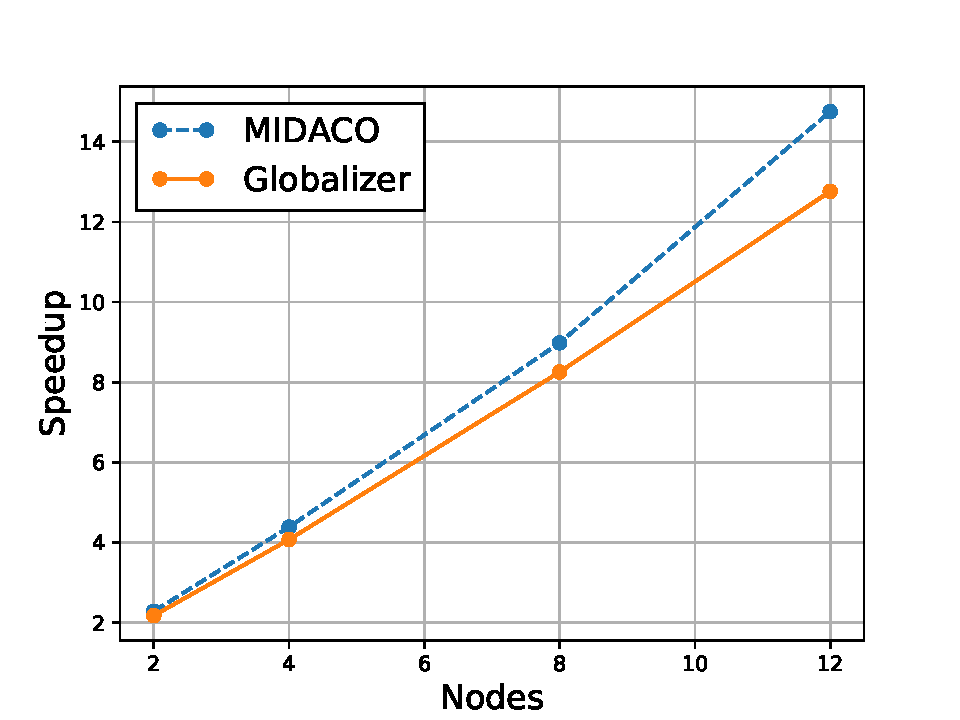
\includegraphics[width=.5\textwidth]{images/speedup_midaco_globalizer_p_1.pdf}}\label{fig:speedup_p1}}
  \subfloat[$p=16$]{{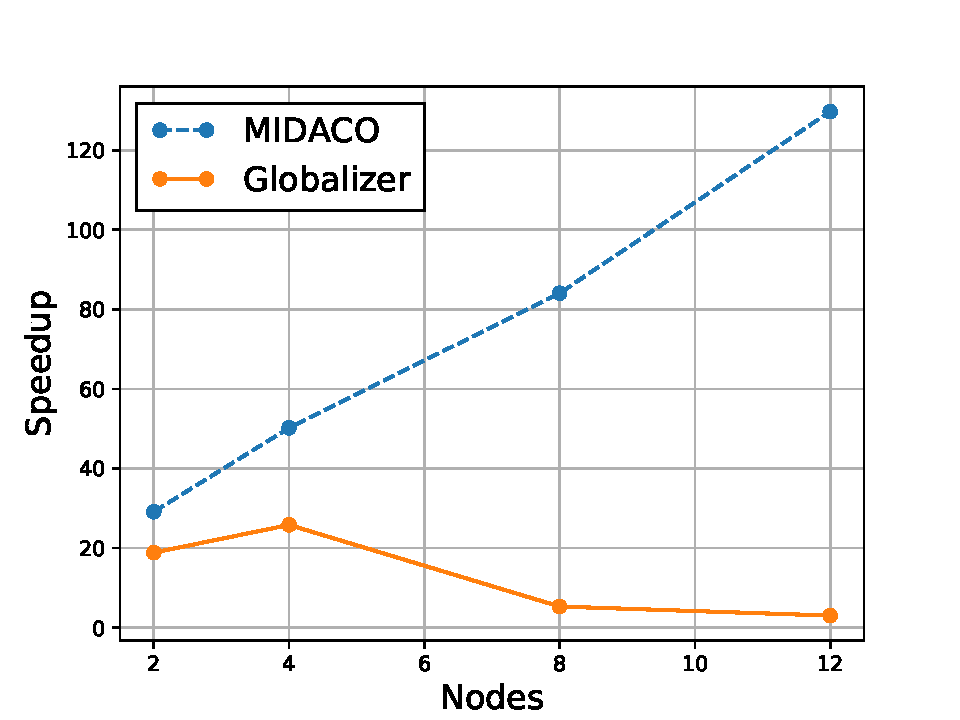
\includegraphics[width=.5\textwidth]{images/speedup_midaco_globalizer_p_16.pdf}}\label{fig:speedup_p16}}
  \caption{Speedup demonstrated by the parallel algorithms when solving problems from the GKLS 4d Hard class}
\end{figure}

\begin{figure}[ht]
  \centering
  \subfloat[$p=1$]{{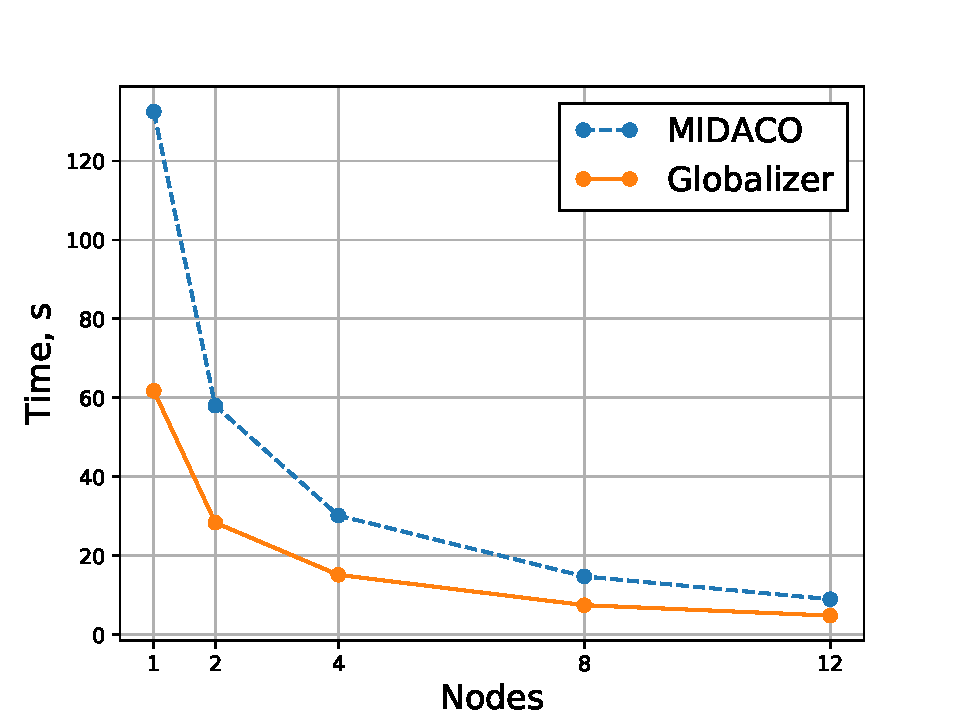
\includegraphics[width=.5\textwidth]{images/time_midaco_globalizer_p_1.pdf}}\label{fig:time_p1}}
  \subfloat[$p=16$]{{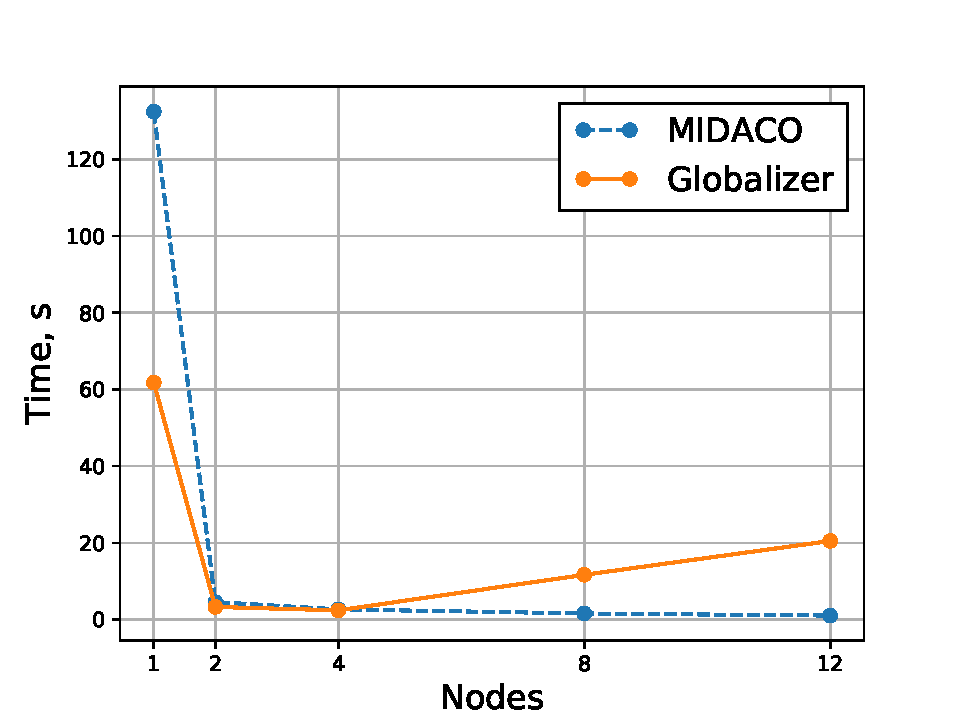
\includegraphics[width=.5\textwidth]{images/time_midaco_globalizer_p_16.pdf}}\label{fig:time_p16}}
  \caption{Averaged execution time of the parallel algorithms when solving problems from the GKLS 4d Hard class}
\end{figure}

\begin{table}
  \centering
  \caption{Speedup of parallel computations executed by the parallel algorithms}
  \label{tab:speedup}
  \begin{tabular}{cccccccc}
    \cline{3-8}\noalign{\smallskip}
    \multicolumn{2}{c}{  } & \textit{p} & \multicolumn{2}{c}{Globalizer} & &
\multicolumn{2}{c}{MIDACO}   \\
    \noalign{\smallskip} \cline{4-5} \cline{7-8}  \noalign{\smallskip}
    \multicolumn{2}{c}{  } & & \textit{Simple} & \textit{Hard} & & \textit{Simple} &
\textit{Hard}  \\
    \noalign{\smallskip}\hline
I  & \textbf{1 cluster node}  %\multirow{3}{*}{}
    & \textit{1}   & 25270 (27.3s) & 55180 (61.8s) & & 27645 (32.2s) & 72068 (132.5s)  \\
  &  & \textit{16} & 14.3(11.7) & 14.9(12.6)  & &  16.9(14.4) & 16.7(14.4) \\
  \hline \noalign{\smallskip}
II  & \textbf{2 cluster nodes}  %\multirow{3}{*}{}
  & \textit{1}      &   1.9(1.9) & 2.4(2.2)  & & 2.6(1.7) & 2.7(2.3) \\
  &   & \textit{16} & 34.5(20.4) & 31.4(18.8) & & 24.5(18.8) & 32.0(29.1) \\
    \noalign{\smallskip}\hline	\noalign{\smallskip}
III  & \textbf{4 cluster nodes}  %\multirow{3}{*}{}
& \textit{1}      & 5.0(4.6) & 4.3(4.1) & & 4.8(3.9) & 4.5(4.4) \\
&   & \textit{16} & 68.8(23.7) & 71.2(25.8) & & 52.3(32.9) & 57.0(50.2) \\
  \noalign{\smallskip}\hline	\noalign{\smallskip}
VI & \textbf{8 cluster nodes} %\multirow{3}{*}{}
& \textit{1}    & 12.0(8.7) & 10.9(8.3) & & 9.7(8.2)    & 7.3(9.0)    \\
& & \textit{16} & 174.1(4.7) & 177.8(5.3) & & 101.6(51.6) & 93.1(84.1) \\
    \noalign{\smallskip}\hline
    V & \textbf{12 cluster nodes} %\multirow{3}{*}{}
    & \textit{1}    & 21.9(11.4)  & 23.0(12.8)  & & 12.4(11.1)  & 12.0(14.8)  \\
    & & \textit{16} & 333.5(2.7) & 347.9(3.0) & & 164.5(82.0) & 183.2(129.7) \\
        \noalign{\smallskip}\hline
  \end{tabular}
\end{table}

\section{Conclusions}

In the present paper, several sequential and parallel global optimization algorithms were considered.
A comparison of efficiencies of these ones has been done on a set of test problems. The results allow
making the following conclusions:
\begin{itemize}
  \item AGS\(l\) method implemented in the Globalizer system has demonstrated the convergence
speed and reliability at the level of \(DIRECT\) and exceeds many other algorithms, the open-access
implementations of which are available;
  \item the stochastic optimization methods inferior to the deterministic ones in the convergence
speed and in reliability. It is manifested especially strongly on more complex multiextremal
problems;
  \item the parallel version of the Globalizer system demonstrates good indicators of speedup in time
when running on several nodes, on each of which a single objective function value per iterations is
computed. When solving the problems with fast computable objective functions and using multiple
threads on the nodes, the indicators of speedup for the Globalizer system degrade with increasing
number of nodes;
  \item the MIDACO system is the most suitable for simple global optimization problems with the
fast-computable objective functions. In this case, MIDACO is reliable enough and provides a linear
speedup with increasing number of nodes and threads executed on these ones in parallel.
\end{itemize}


\section*{Acknowledgements}
The study was supported by the Russian Science Foundation, project No 16-11-
10150.

% ---- Bibliography ----
%
\bibliographystyle{spmpsci}
\bibliography{bibliography}{}

\end{document}
